\glsresetall

% Don't show subsections in the TOC.
\addtocontents{toc}{\protect\setcounter{tocdepth}{1}}

The purpose of this chapter is to an provide initial, low-level validation of the model library.  It presents some basic examples of the model introduced in Chapters~\ref{chap:Fundamentals} and~\ref{chap:Implementation}.  Each section begins with an introduction of the physical conditions and assumptions.  Then, simulation results are shown and discussed.  Most of the examples in this chapter are not intended to be representative of a fuel cell.  However, the last two examples demonstrate phase change processes which are scaled so that the time constants roughly correspond to a \n{PEMFC}.

It is significant that all of the following examples---from gas dynamics to electrical con\-duction---were generated from the same working model (\modelica{Subregion}), only instantiated with various geometries and initial and boundary conditions.  The models of solids, liquid water, gases, electrons, and protons are different only in their material properties and default assumptions, all of which are configurable.

In addition to these examples, a comprehensive package of test models was created and simulated  to verify the thermodynamic and transport properties of the fluids against~\cite{Moran2004} and~\cite{Incropera2002}.  Also, the physical constants were verified against~\cite{NIST2010}.

The results of each example begins with statistics about the model and its simulation.  The models contain a number of variables, some of which are time-varying.  The number of states is the number of time derivatives that are algebraically independent.  It is the number of unique ways that energy can be introduced and stored in a model (enthalpy of formation between phases, boundary work, energy due to charge displacement, kinetic energy along each axis, and internal energy).  At a given time, the state variables can be considered known.  The size of each system of equations is the number of algebraically coupled equations that must be solved from the known variables, which include the states and time-constant variables.  The systems of equations may be linear or nonlinear.

Before simulation, a model must be translated.  This includes the process of parsing the Modelica syntax, flattening the object-oriented code, manipulating and sorting the equations, tearing systems of equations, and compiling the result with links to the solvers and integrator.  The models were translated and simulated on a Samsung ATIV Book 8 laptop computer (Intel Core i7 3635QM @ \SI{2.40}{GHz}, \SI{8}{GB}~RAM DDR3 @ \SI{1600}{MHz}, \SI{5400}{RPM}~hard drive) running Windows~8.1 and Dymola~2014.  The hardware represents technology that is approximately one year old (processor introduced 3\textsuperscript{rd} quarter 2012). 

The default Dymola settings were used, including the \n{DASSL} and 500 output intervals, except:
\begin{enumerate*}
  \item \modelica{GuardedSqrt = false}
  \item \modelica{ImprovedPackageConstants = true}
  \item \modelica{IncludeLibrariesForSimulink = false}
  \item \modelica{SubstituteVariablesUsedOnce = true}
\end{enumerate*}
Most models were simulated with an integration tolerance of \num{E-4}, but this was increased as needed.  The following debugging options were enabled which may have affected the translation and compilation time:
\begin{enumerate*}
  \item \modelica{CheckUnits = false}
  \item \modelica{LogDefaultInitialConditions = true}
  \item \modelica{LogStateSelection = true}
  \item \modelica{OutputCPUtime = true}
  \item \modelica{OutputModelicaCode = true}
  \item \modelica{OutputModelicaCodeWithAliasVariables = true}
  \item \modelica{StoreProtectedVariables = true}
\end{enumerate*}



\section{Internal Flow}
\label{sec:InternalFlow}

This example compares the model to Poiseuille's law~\cite{Cengel2006} for pressure drop along a pipe under laminar flow.  Poiseuille's law was derived from the model equations in \autoref{sec:TransverseTransport}, so this example is partly a test that the implementation performs as expected.  It also demonstrates inertance and thermal dynamics.

\subsection{Conditions}

Liquid water is forced along the long axis through a rectangular $\SI{1}{m}\times\SI{1}{mm}\times\SI{1}{mm}$ subregion as shown in \autoref{fig:InternalFlow}.  In addition to a large-signal volumetric flow rate of \SI{1.5}{cm^3/s}, there is a small sinusoidal signal with an amplitude of \SI{0.3}{cm^3/s} and a frequency of \SI{1}{Hz}.  This corresponds to an area-average (plug flow equivalent) velocity of $1.5\pm$\SI{0.3}{m/s} as shown in \autoref{fig:InternalFlowRate}. % and a space velocity of $1.5\pm$\SI{0.3}{s^{-1}}.  
A no-slip (zero velocity) condition is applied around the perimeter.  The fluid source is held at \SI{25}{\celsius}.  There is no thermal conduction across the outlet (only advection) or around the perimeter.  

\begin{figure}[htbp]
  \subfloat[Physical domain]{
    \fbox{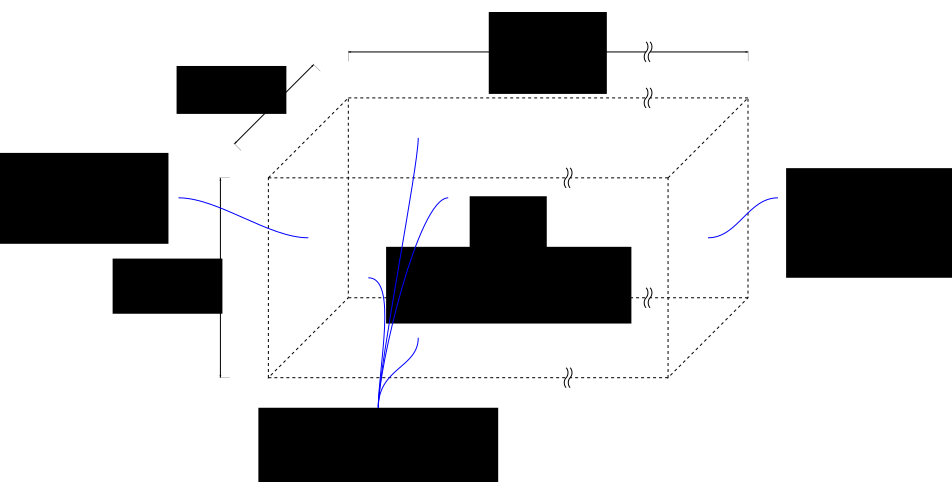
\includegraphics[width=\linewidth]{5-InternalFlow}}%
    \label{fig:InternalFlowPhysical}
  }\\
  \subfloat[Model]{
    \fbox{\includegraphics[width=0.6\linewidth]{5-InternalFlowD}}%
    \label{fig:InternalFlowDiagram}
  }
  \caption{Configuration of the internal flow example}\glsadd{IC}
  \label{fig:InternalFlow}
\end{figure}

\begin{figure}[htbp]
  \includegraphics[width=\linewidth]{Results/Basic/InternalFlow/1/Velocity}%
  \caption{Fluid velocity for the internal flow example}%
  \label{fig:InternalFlowRate}
\end{figure}

The Reynolds number varies from 1400 to 2100; therefore, laminar flow is expected.  The translational Nusselt number for the liquid water is set to four ($\s{Nu}[_Phi] = 4$, the default), which is appropriate for laminar flow with a single subregion over the cross section.

\subsection{Results and Discussion}

\begin{table}[h]
  \caption{Modeling and simulation statistics for the internal flow example}
  \begin{singlespaced}%
    \begin{tabular}{llll}%
      \toprule 
      & With analysis & Without analysis \\
        \midrule
      Number of variables & 516 & 474 \\
      Number of time-varying variables & 104 & 55 \\
      Number of states & 1 & 1 \\
      Sizes of the nonlinear systems of equations & None & None \\
      Sizes of the linear systems of equations & 4 sets of 2 & 4 sets of 2 \\
      Translation time & \SI{3}{s} & \SI{1}{s} \\
      Simulation time & \SI{0.007}{s} & \SI{0.007}{s} \\
      \bottomrule
    \end{tabular}
  \end{singlespaced}
\end{table}



The modeling and simulation statistics are listed above.  The model contains a fairly large number of variables (516) given the simple physical system.  The object-oriented nature of the model introduces overhead in terms of the number of variables.  Some of the variables (8\% of all variables and 47\% of the time-varying variables) are outputs that are purely for analysis.  They can be disabled without affecting the behavior.  Roughly one fifth of the variables are time-varying.  The model contains only one state: temperature.  Velocity is not a state since the translational dynamics are imposed directly by the boundary conditions (prescribed volumetric flow rate) and the fluid is incompressible.  There are no time-varying systems of algebraic equations after manipulation.  The model simulates very quickly (\SI{7}{ms}). The analysis variables have negligible effect on the simulation time.  Translation takes over 400~times longer than simulation.  However, the model may be re-simulated with various parameter settings without re-translating it.

\autoref{fig:InternalFlowPressure} shows the difference in thermodynamic pressure across the subregion.  Due to inertance, the pressure difference of the model leads the pressure difference according to Poiseuille's law and has a slightly larger amplitude.  The effect of inertance becomes more prominent at higher frequencies and less so at lower frequencies.

\begin{figure}[htbp]
  \includegraphics[width=\linewidth]{Results/Basic/InternalFlow/1/Pressure}%
  \caption{Dynamic pressure difference under internal flow}%
  \label{fig:InternalFlowPressure}
\end{figure}

The temperature of the fluid in the subregion increases due to viscous dissipation as shown in \autoref{fig:InternalFlowTemperature}.  However, the temperature rise is only \SI{9}{mK} (to \SI{25.009}{\celsius}) because the rate of heat generation is much smaller than the rate of enthalpy flow from the source.  The increase is so slight that the simulation tolerance must be increased from $10^{-4}$ (the default) to $10^{-8}$ in order to distinguish it from the solver error.  The temperature increases with a first-order dynamic response.  A sinusoidal temperature variation is superimposed due to the small-signal part of the flow rate.  

\begin{figure}[htbp]
  \includegraphics[width=\linewidth]{Results/Basic/InternalFlow/1/Temperature}%
  \caption{Thermal transients due to viscous dissipation in internal flow}%
  \label{fig:InternalFlowTemperature}
\end{figure}


\FloatBarrier % Flush the floats.
\section{Echo}

This example shows the dynamics of compressible flow in the model.  A pressure wave reflects between the external boundaries of adjacent subregions.  The effect of the discretization scheme can be seen.  The key model equations are material transport (\autoref{eq:MaterialTransport}) and material conservation (\autoref{eq:MaterialBalance}).

\subsection{Conditions}

Two cubic \SI{1}{cm^3} subregions containing \n{H2} are arranged side-by-side with an initial pressure difference of \SI{100}{Pa} as shown in \autoref{fig:Echo}.  The \modelica{subregions} array of models is removed and bypassed upon translation because there are only two subregions.  Both subregions are initialized to \SI{25}{\celsius}.  All external boundaries are isolated (i.e., closed, adiabatic, and free-slip).  The model is evaluated with upstream discretization and with the central difference scheme.

\begin{figure}[htbp]
  \subfloat[Physical domain]{
    \fbox{\includegraphics[width=3in]{5-Echo}}%
    \label{fig:EchoPhysical}
  }\vspace*{-1.6cm}\\\includegraphics[width=4in]{5-EchoLink}\vspace*{-4cm}\\
  \subfloat[Model]{
    \fbox{\includegraphics[width=0.6\linewidth]{5-EchoD}}%
    \label{fig:EchoDiagram}
  }
  \caption{Configuration of the echo example (\s{H2} gas with an initial pressure difference)}
  \label{fig:Echo}
\end{figure}

\subsection{Results and Discussion}

\begin{table}[h]
  \caption{Modeling and simulation statistics for the echo example}
  \begin{singlespaced}%
    \begin{tabular}{llll}%
      \toprule 
      & Upstream & Central \\
      & discretization & difference \\
        \midrule
      Number of variables & 488 & 488 \\
      Number of time-varying variables & 122 & 118 \\
      Number of states & 5 & 5 \\
      Sizes of the nonlinear systems of equations & None & None \\
      Sizes of the linear systems of equations & 2 sets of 2 & 2 sets of 2 \\
      Translation time & \SI{3}{s} & \SI{3}{s} \\
    Simulation time & \SI{0.011}{s} & \SI{0.010}{s} \\
      \bottomrule
    \end{tabular}
  \end{singlespaced}
\end{table}



The model simulates slightly faster (9\%) with the central difference scheme, although the time may not be significant given the uncertainty due to the overhead of the operating system.  These models are roughly the same as the internal flow model (\autoref{sec:InternalFlow}) in terms of complexity, translation time, and simulation time.

As shown in \autoref{fig:EchoPressureDamped}, the model exhibits oscillations due to the coupled dynamics of compression and translation.  This is essentially a mass-spring-damper system.  The damping is due to irreversible material compression and expansion (\autoref{eq:MaterialTransport}).  If the continuity (\s{zeta}) is set to zero, there is no damping.  This case is shown in \autoref{fig:EchoPressureNoDamping}.  The outer boundaries have the same temperature as the nearest subregion.  The period of oscillation is \SI{0.0338}{ms}, which corresponds to a wave velocity of \SI{592}{m/s}.  This is roughly half of the speed that is expected for \n{H2} as an ideal gas at \SI{25}{\celsius} with an adiabatic index of approximately 1.4.  Currently, the reason for the discrepancy is unknown.  The plots in \autoref{fig:EchoPressure} are from the case where upstream discretization is used, but the central difference scheme gives identical results.  The common boundary remains at the average pressure in both cases.  An upstream bias is applied to the balance between pressure gradients and irreversible compression, but the associated P\'eclet number is very small even with the significant damping evident in \autoref{fig:EchoPressureDamped}.  For incompressible fluids, the damping and the P\'eclet number is exactly zero.

\begin{figure}[htbp]
  \subfloat[Default damping]{
    \includegraphics[width=\linewidth]{Results/Basic/Echo/2/Pressure}%
    \label{fig:EchoPressureDamped}
  }\quad
  \subfloat[No damping]{
    \includegraphics[width=\linewidth]{Results/Basic/Echo/3/Pressure}%
    \label{fig:EchoPressureNoDamping}
  }
  \caption{Pressure dynamics in the echo example}
  \label{fig:EchoPressure}
\end{figure}

Due to thermodynamics, the temperature of the first subregion decreases as its gas expands and the temperature of the second subregion increases as it is compressed.  The changes in temperature are small because the thermal effect is secondary to the main effect of pressure equalization.  As shown in \autoref{fig:EchoTemperature}, the temperature at the common boundary depends on the discretization scheme.  According to upstream discretization, the temperature of the common boundary is biased by the source (\autoref{fig:EchoTemperatureUpstream}).  There is no such bias with the central difference scheme (\autoref{fig:EchoTemperatureCentral}).  Both of these plots are with the default value of continuity ($\s{zeta} = \SI{2.32E-5}{N/A}$).  Since the outer boundaries are adiabatic, the temperature at the outer boundaries are equal to the temperature of the nearest subregion.  At the end of these plots (\SI{0.05}{ms}), the temperatures of the regions are different, yet there is very little thermal convection because the velocities have decayed to nearly zero.  Over a much longer period (\SI{2.5}{s}), the temperatures equalize due to thermal conduction, as shown in \autoref{fig:EchoTemperatureLong}.  The long-term trend of temperature is the same for upstream discretization and the central difference scheme.

\begin{figure}[htbp]
  \subfloat[Upstream discretization]{
    \includegraphics[width=\linewidth]{Results/Basic/Echo/2/Temperature}%
    \label{fig:EchoTemperatureUpstream}
  }\quad
  \subfloat[Central difference scheme]{
    \includegraphics[width=\linewidth]{Results/Basic/Echo/5/Temperature}%
    \label{fig:EchoTemperatureCentral}
  }
  \caption{Temperature oscillations in the echo example}
  \label{fig:EchoTemperature}
\end{figure}

\begin{figure}[htbp]
  \includegraphics[width=\linewidth]{Results/Basic/Echo/1/Temperature}%
  \caption{Long-term thermal equilibration in the echo example}
  \label{fig:EchoTemperatureLong}
\end{figure}

Gas travels in the positive direction due to the initial pressure difference and then returns due to compression, as shown in \autoref{fig:EchoVelocity}.  Although it is not apparent in \autoref{fig:EchoVelocityDampened}, the magnitude of the velocity is slightly greater in the second subregion because that subregion initially has less mass and therefore greater acceleration from a given pressure difference.  This is shown in \autoref{fig:EchoVelocityZoom}.  The plots are for the case of upstream discretization, but the central difference scheme gives identical results.

\begin{figure}[htbp]
  \subfloat[Dampened oscillation]{
    \includegraphics[width=\linewidth]{Results/Basic/Echo/2/Velocity}%
    \label{fig:EchoVelocityDampened}
  }\quad
  \subfloat[Close-up of first crest]{
    \includegraphics[width=\linewidth]{Results/Basic/Echo/2/VelocityZoom}%
    \label{fig:EchoVelocityZoom}
  }
  \caption{Velocity in the echo example}
  \label{fig:EchoVelocity}
\end{figure}


\FloatBarrier % Flush the floats.
\section{Air Column}

This example shows the effect of body forces on a gas.  Like the previous example, it exhibits oscillations due to the coupled dynamics of translation and compression.  The key model equations are material transport (\autoref{eq:MaterialTransport}), material conservation (\autoref{eq:MaterialBalance}), and the translational momentum balance (\autoref{eq:TranslationalBalance}).

\subsection{Conditions}

A vertical column of five \SI{10 x 10 x 10}{m} subregions contain \n{N2} gas (roughly representing air), as shown in \autoref{fig:AirColumn}.  The gas is initialized uniformly to \SI{25}{\celsius} and \SI{1}{bar}.  The external boundaries are isolated (i.e., closed, adiabatic, and free-slip) except for the upper boundary which is held at \SI{25}{\celsius} and \SI{1}{bar}.  Standard gravity is applied (\SI{9.81}{m/s^2}).  The central difference scheme is used.

\begin{figure}[htbp]
  \subfloat[Physical domain]{
    \fbox{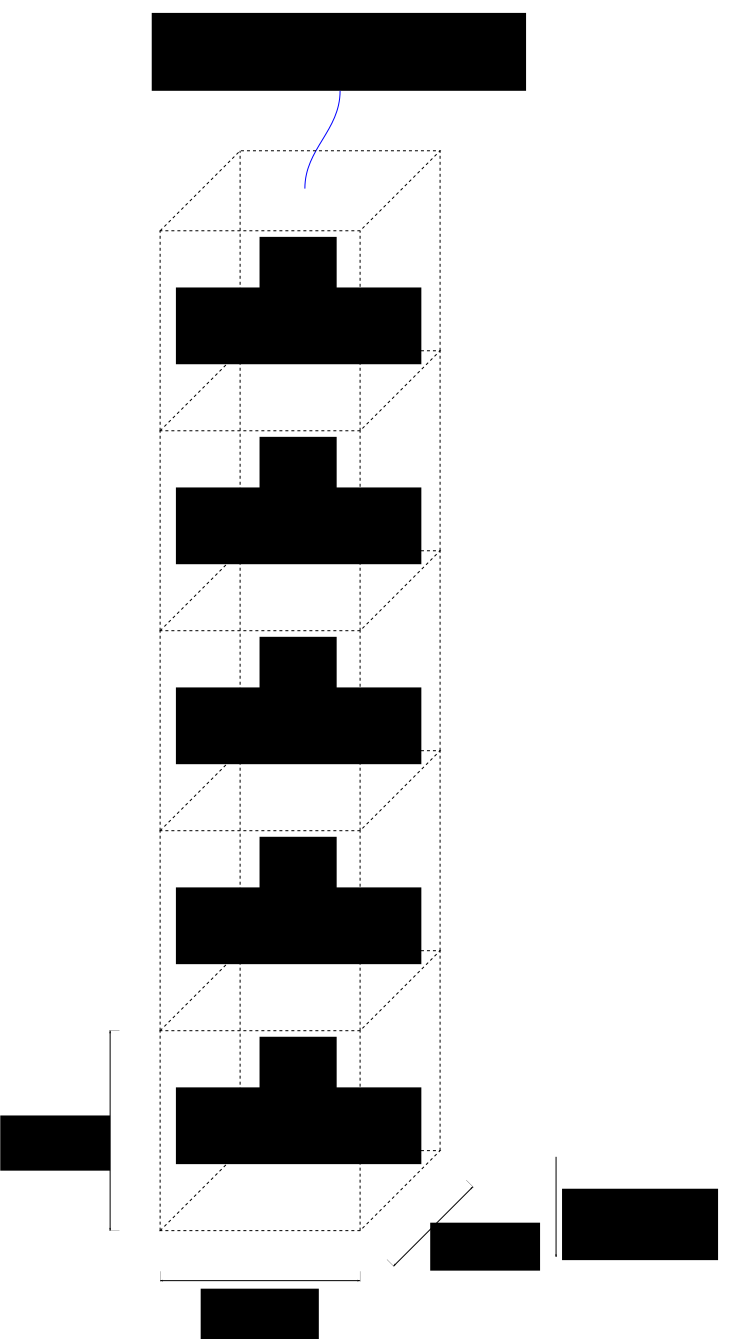
\includegraphics[height=4.4in]{5-AirColumn}}%
    \label{fig:AirColumnPhysical}
  }\hspace*{-3.2cm}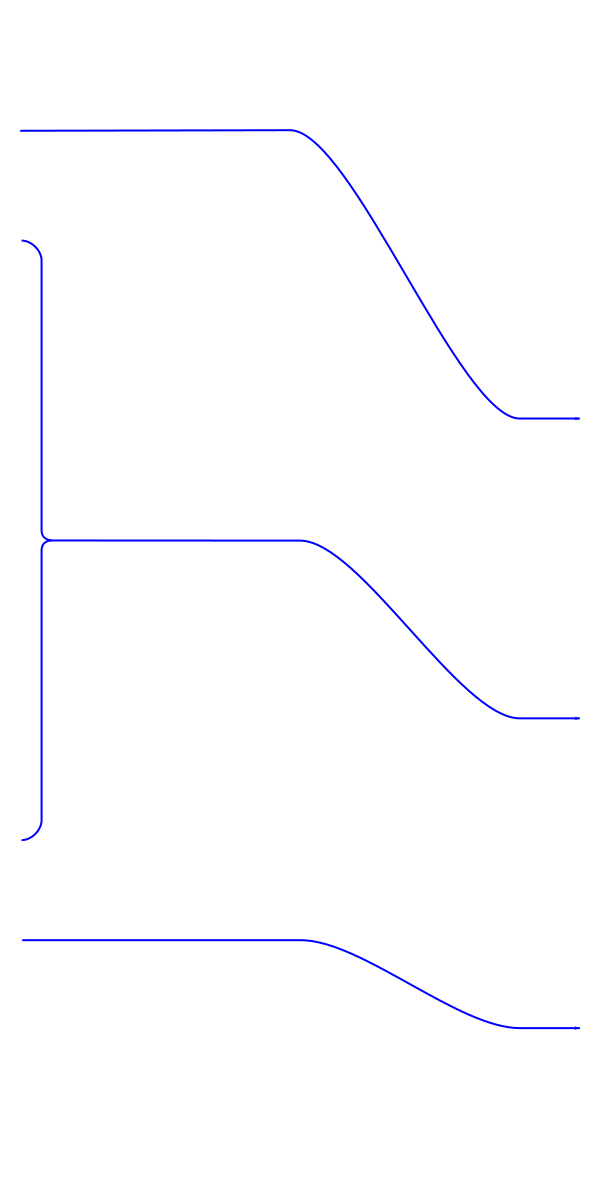
\includegraphics[height=3.9in]{5-AirColumnLink}\hspace*{-1.3cm}
  \subfloat[Model]{
    \fbox{\includegraphics[height=3.7in]{5-AirColumnD}}%
    \label{fig:AirColumnDiagram}
  }
  \caption{Configuration of the air column example (gas under the influence of gravity)}
  \label{fig:AirColumn}
\end{figure}

\subsection{Results and Discussion}

\begin{contextbox}
  Modeling and simulation statistics:
  \begin{itemize}
    \item Number of variables: 1168
    \item Number of time-varying variables: 284
    \item Number of states: 15
    \item Sizes of the nonlinear systems of equations: None
    \item Sizes of the linear systems of equations: 8 sets of 2
    \item Translation time: \SI{3}{s}
    \item Simulation time: \SI{0.016}{s}
  \end{itemize}
\end{contextbox}

This model has roughly twice as many variables as the previous examples, yet it translates and simulates in about the same time.  There are 15 states---the temperature, pressure, and vertical component of velocity in each of the five subregions.

The total pressure difference over all the subregions is plotted in \autoref{fig:AirColumnPressureDifference}.  It oscillates due to the dynamics of translation and compression.  It takes approximately \SI{3}{s} for the pressure difference to settle to the expected value---the product of density, acceleration due to gravity, and column height ($\s{m}\s{rho}\s{a}[_y]\s{L}[_y]$).  \autoref{fig:AirColumnPressureDistribution} shows that the pressure gradient is uniform at steady state, as expected.

\begin{figure}[htbp]
  \subfloat[Total pressure difference]{
    \includegraphics[width=\linewidth]{Results/Basic/AirColumn/2/PressureDifference}%
    \label{fig:AirColumnPressureDifference}
  }\quad
  \subfloat[Pressure distribution]{
    \includegraphics[width=\linewidth]{Results/Basic/AirColumn/2/Pressure}%
    \label{fig:AirColumnPressureDistribution}
  }
  \caption{Pressure in the air column example}
  \label{fig:AirColumnPressure}
\end{figure}

As shown in \autoref{fig:AirColumnVelocity}, the gas accelerates downward and then rebounds upward due to compression.  The maximum downward velocity is approximately \SI{85}{cm/s} at the upper boundary.

\begin{figure}[htbp]
  \includegraphics[width=\linewidth]{Results/Basic/AirColumn/2/Velocity}%
  \caption{Velocity transients in the air column example}
  \label{fig:AirColumnVelocity}
\end{figure}

The temperatures of the subregions increase due to the adiabatic compression, as shown in \autoref{fig:AirColumnTemperatureShort}.  This develops a temperature gradient where the lower subregions are slightly hotter.  In reality, this would lead to natural convection.  However, in this idealized model, there is only one transport path and no way for a circulation cell to develop.  Therefore, the temperature can only equalize by conduction.\footnote{The model also assumes no thermal radiation.}  The time constants, which are calculated as output variables of the model and plotted in \autoref{fig:AirColumnTimeConstants}, are approximately 19~days for transport from a boundary into a subregion due to the size of the system and the properties of the gas.  These large time constants do in fact match the theoretical result. \autoref{fig:AirColumnTemperatureLong} shows the long-term temperature trends.  The full equalization takes approximately three years.  While this example is rather academic, it demonstrates the stability and flexibility of the model and the solver.  The same translated model was used for both the short- and long-term simulations---a ratio of \num{31557600} in simulated time---with roughly the same computation time (16 and \SI{19}{ms}).

\begin{figure}[htbp]
  \subfloat[Initial oscillations]{
    \includegraphics[width=\linewidth]{Results/Basic/AirColumn/2/Temperature}%
    \label{fig:AirColumnTemperatureShort}
  }\quad
  \subfloat[Equalization over the long term]{
    \includegraphics[width=\linewidth]{Results/Basic/AirColumn/1/Temperature}%
    \label{fig:AirColumnTemperatureLong}
  }
  \caption[Thermal transients in the air column example]{Thermal transients in the air column example.  Since the boundaries are adiabatic, the temperatures of the lower and upper boundaries (not plotted) are equal to the temperatures of subregions 1 and 5}
  \label{fig:AirColumnTemperature}
\end{figure}

\begin{figure}[htbp]
  \includegraphics[width=\linewidth]{Results/Basic/AirColumn/1/TimeConstants}%
  \caption{Thermal time constants in the air column example}
  \label{fig:AirColumnTimeConstants}
\end{figure}


\FloatBarrier % Flush the floats.
\section{Electrical Conduction}

This is an example of Ohm's law with thermal dynamics.  The key equations are translational exchange (\autoref{eq:TranslationalDiffusiveExchange}), thermal conduction (\autoref{eq:ThermalDiffusiveTransport}), and the energy balance (\autoref{eq:EnergyBalanceIntensive}).

\subsection{Conditions}

A $\SI{1}{m}\times\SI{1}{mm}\times\SI{1}{mm}$ block of graphite is held at \SI{25}{\celsius}, as shown in \autoref{fig:ElectricalConduction}.  An electrical current ($\s{z}{I}$) of \SI{50}{mA} is pulled from the negative boundary (\s{e-} into the boundary), and the positive boundary is held at a reference electronic pressure\slash{}potential.  The electrical conductivity (\s{sigma}) is \SI{100}{S/m}.  The perimeter is closed and adiabatic.

\begin{figure}[htbp]
  \subfloat[Physical domain]{
    \fbox{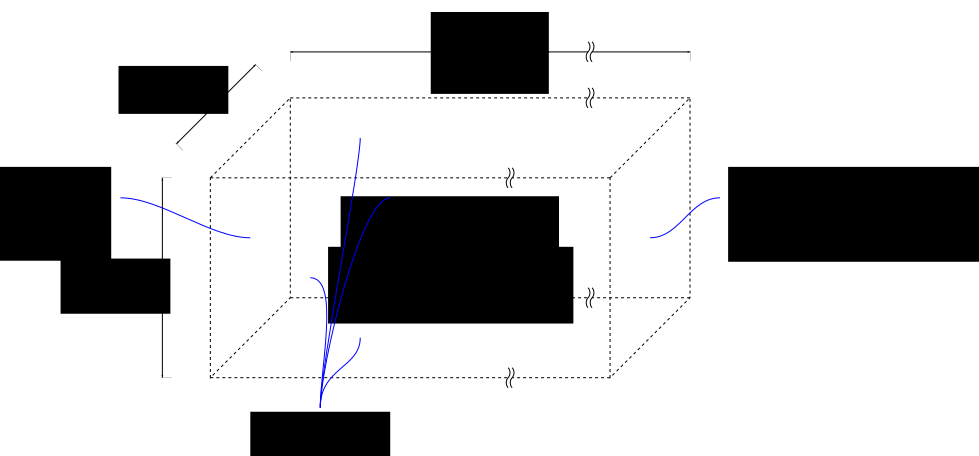
\includegraphics[width=\linewidth]{5-ElectricalConduction}}%
    \label{fig:ElectricalConductionPhysical}
  }\\
   \subfloat[Model]{ 
\fbox{\begin{minipage}{0.5\linewidth}
    \includegraphics[width=\linewidth, clip, trim=0 110 0 0]{5-ElectricalConductionD}\\
    \includegraphics[width=\linewidth, clip, trim=0 0 0 130]{5-ElectricalConductionD}%
\end{minipage}}
    \label{fig:ElectricalConductionDiagram}
  }
  \caption{Configuration of the electrical conduction example}
  \label{fig:ElectricalConduction}
\end{figure}

\subsection{Results and Discussion}

\begin{contextbox}
  Modeling and simulation statistics:
  \begin{itemize}
    \item Number of variables: 31990
    \item Number of time-varying variables: 12711
    \item Number of states: 266
    \item Sizes of the nonlinear systems of equations: None
    \item Translation time: \SI{69}{s}
    \item Simulation time: \SI{11.3}{s}
  \end{itemize}
\end{contextbox}

As expected, the simulation shows an electrical resistance of $\s{R} = \s{L}/\s{sigma}\s{A} = \SI{100}{\ohm}$.  The rate of heat generation is $\dot{Q}[_gen] = (\s{z}{I})^2\s{R} = \SI{250}{mW}$.  

\autoref{fig:ElectricalConductionTemperature} shows the temperature trend.  As expected, the steady-state temperature is $\s{T} = \s{T}_0 + \s{theta}\s{L}\dot{Q}[_gen]/4\s{A} \approx \SI{82}{\celsius}$, where $\s{T}_0$ is the boundary temperature (\SI{25}{\celsius}), \s{theta}~is the thermal resistance, \s{L}~is the length (\SI{1}{cm}), and \s{A}~is the cross-sectional area (\SI{1}{mm^2}).  The factor of one fourth is due to the boundary conditions; the conduction length is half of the total length and the heat is rejected to both sides.  The time constant, as measured by the time to $1 - e^{-1} (\approx 63\%$) of the final value, is approximately equal to $\s{tau}\sub{_Q}[_T]/2$, were $\s{tau}\sub{_Q}[_T]$~is the time constant for thermal conduction from one side into the subregion (\autoref{eq:TimeConstantThermalTransport}).

\begin{figure}[htbp]
  \includegraphics[width=\linewidth]{Results/Basic/ElectricalConduction/Temperature}%
  \caption{Dynamic heating of an electrical resistor}%
  \label{fig:ElectricalConductionTemperature}
\end{figure}


\FloatBarrier % Flush the floats.
\section{Thermal Conduction}
\label{sec:ThermalConduction}

This example demonstrates distributed thermal conduction and heating.  The key model equations are thermal conduction (\autoref{eq:ThermalDiffusiveTransport}) and the energy balance (\autoref{eq:EnergyBalanceIntensive}).

\subsection{Conditions}
\label{sec:ThermalConductionConditions}

A graphite bar divided into eight \SI{1}{cm^3} subregions, as shown in \autoref{fig:ThermalConduction}.  The initial temperature of the first subregion is \SI{55}{\celsius}; the others begin at \SI{25}{\celsius}.  The outer boundaries are adiabatic.

\begin{figure}[htbp]
  \subfloat[Physical domain]{
    \fbox{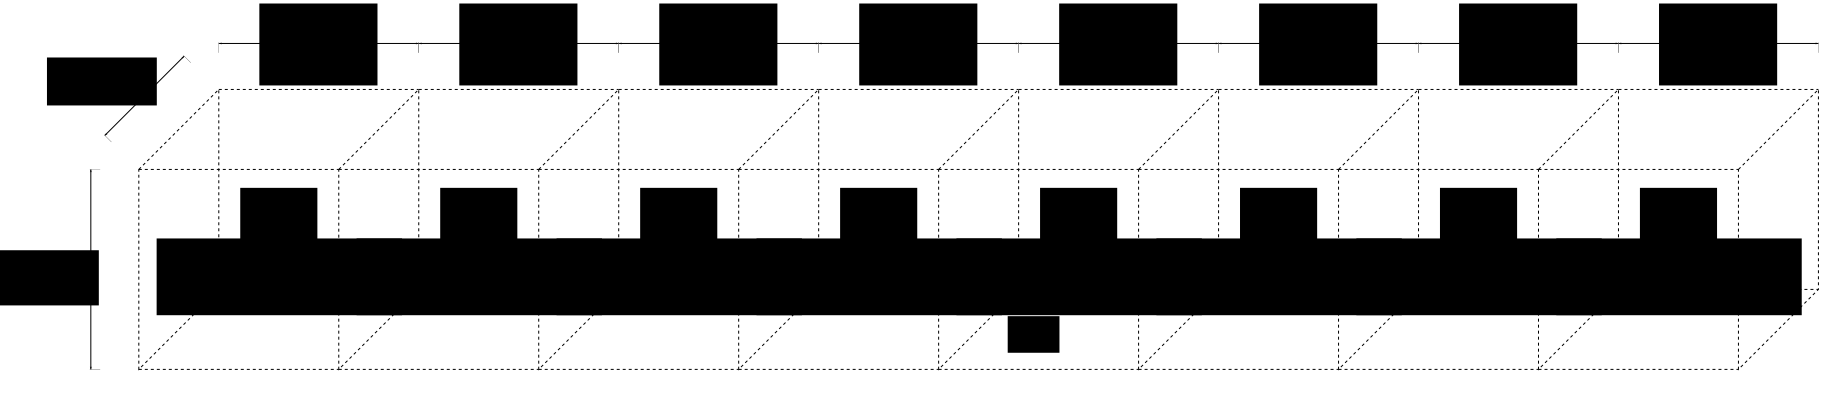
\includegraphics[width=\linewidth]{5-ThermalConduction}}%
    \label{fig:ThermalConductionPhysical}
  }\vspace*{-1.72cm}\\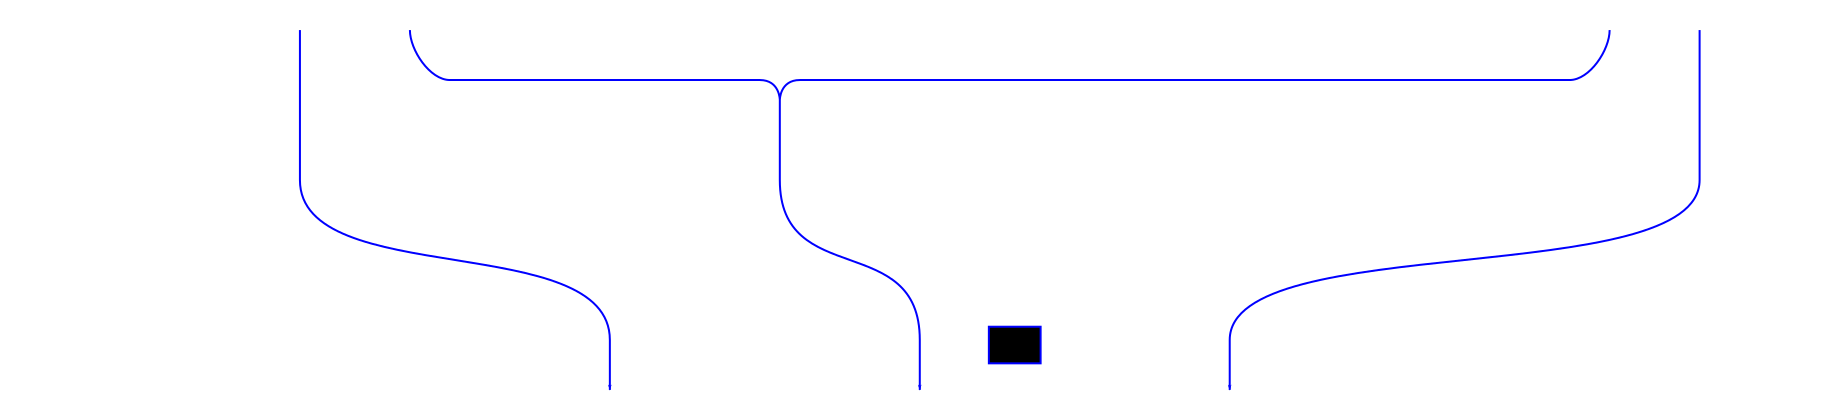
\includegraphics[width=\linewidth]{5-ThermalConductionLink}\vspace*{-1cm}\\
  \subfloat[Model]{
    \fbox{\includegraphics[width=0.6\linewidth]{5-ThermalConductionD}}%
    \label{fig:ThermalConductionDiagram}
  }
  \caption{Configuration of the thermal conduction example}
  \label{fig:ThermalConduction}
\end{figure}

\subsection{Results and Discussion}

\begin{contextbox}
  Modeling and simulation statistics:
  \begin{itemize}
    \item Number of variables: 1119
    \item Number of time-varying variables: 80
    \item Number of states: 8
    \item Sizes of the nonlinear systems of equations: None
    \item Sizes of the linear systems of equations: 7 sets of 2
    \item Translation time: \SI{3}{s}
    \item Simulation time: \SI{0.009}{s}
  \end{itemize}
\end{contextbox}

\autoref{fig:ThermalConductionTemperature} shows the temperature trends throughout the graphite bar.  The temperatures distribute evenly and then converge to a final temperature of approximately \SI{28}{\celsius} after \SI{500}{s}.  Since there is no material transport, the temperatures of the interfaces are the average temperatures of the neighboring subregions.  

\begin{figure}[htbp]
  \includegraphics[width=\linewidth]{Results/Basic/ThermalConduction/Temperature}%
  \caption{Temperature in a graphite bar during transient conduction}%
  \label{fig:ThermalConductionTemperature}
\end{figure}


\FloatBarrier % Flush the floats.
\section{Thermal Conduction and Convection}
\label{sec:ThermalConductionConvection}

This example builds on the previous one.  It adds gas to the system and shows how the gas moves as the temperature equalizes.  Material transport (\autoref{eq:MaterialTransport}) and translational exchange (\autoref{eq:TranslationalDiffusiveExchange}) are important here.

\subsection{Conditions}

The conditions are the same as described in \autoref{sec:ThermalConductionConditions}, except that \n{N2} gas now occupies half of the volume of each subregion.  The gas is initialized to \SI{1}{atm} and the same temperature as the solid.  Initially, it has zero velocity.  The translational independence factor is ten ($\s{k}\sub{_Phi}[_x] = 10$), which represents a porous media.

\begin{figure}[htbp]
  \subfloat[Physical domain]{
    \fbox{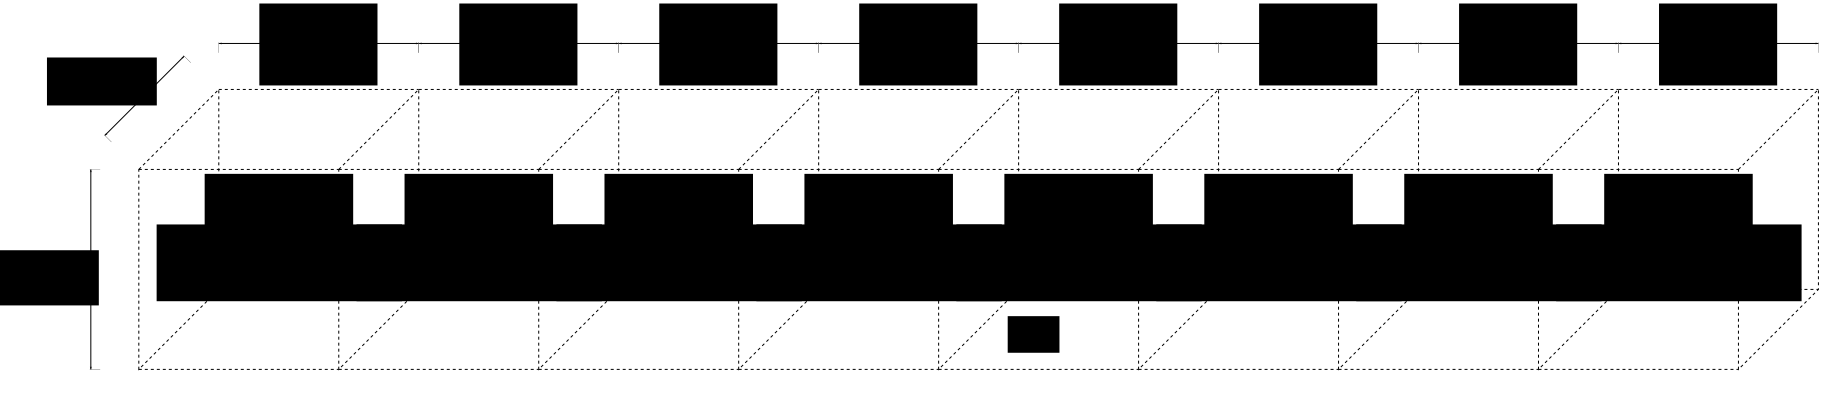
\includegraphics[width=\linewidth]{5-ThermalConductionConvection}}%
    \label{fig:ThermalConductionConvectionPhysical}
  }\vspace*{-1.72cm}\\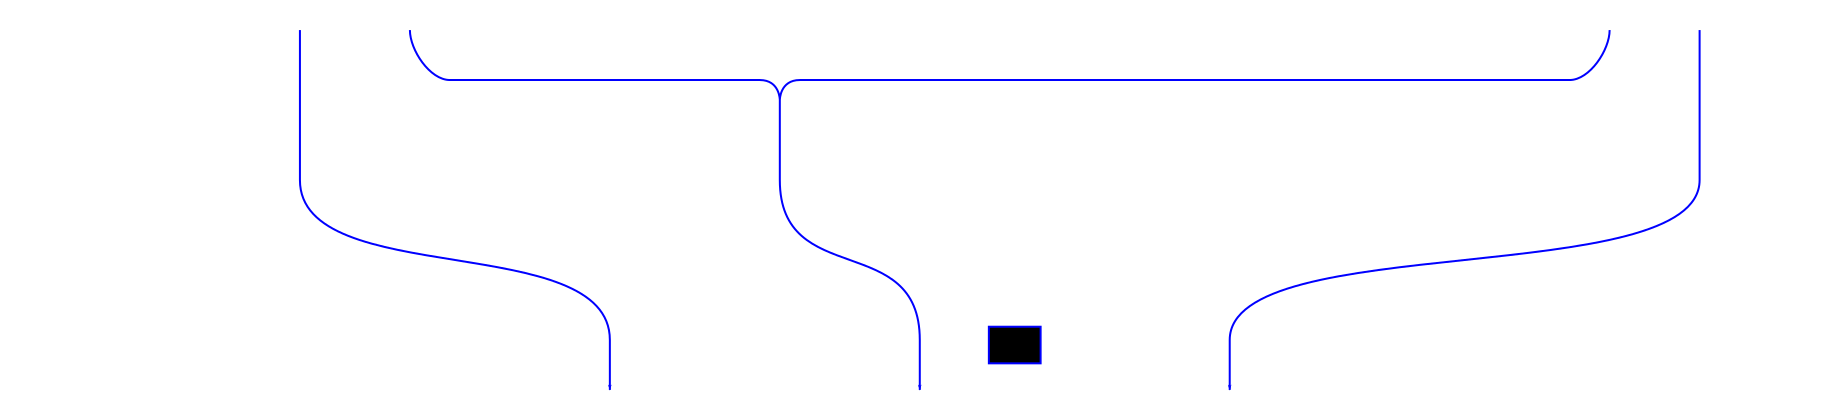
\includegraphics[width=\linewidth]{5-ThermalConductionLink}\vspace*{-1cm}\\
  \subfloat[Model]{
    \fbox{\includegraphics[width=0.6\linewidth]{5-ThermalConductionConvectionD}}%
    \label{fig:ThermalConductionConvectionDiagram}
  }
  \caption{Configuration of the thermal conduction and convection example}
  \label{fig:ThermalConductionConvection}
\end{figure}

\subsection{Results and Discussion}

\begin{contextbox}
  Modeling and simulation statistics:
  \begin{itemize}
    \item Number of variables: 2407
    \item Number of time-varying variables: 574
    \item Number of states: 31
    \item Sizes of the nonlinear systems of equations: None
    \item Sizes of the linear systems of equations: 43 sets of 2
    \item Translation time: \SI{5}{s}
    \item Simulation time: \SI{0.072}{s}
  \end{itemize}
\end{contextbox}

The simulation is approximately eight times slower than the example without the gas (\autoref{sec:ThermalConduction}).  There are states for the temperature of the solid and the temperature and pressure of the gas in every subregion (24 states).  There are also states for the x component of velocity in all but one subregion (7 states).  One of the translational states is eliminated due to the closed outer boundaries.

The temperature trends are nearly the same as for the previous example (\autoref{fig:ThermalConductionTemperature}).  The gas and the solid remain at approximately the same temperature in each subregion.  

Due to the equation of state, the gas in the first subregion becomes denser and has lower pressure as it becomes colder.  This is shown in Figures~\ref{fig:ThermalConductionConvectionVelocity} and \ref{fig:ThermalConductionConvectionPressure}.  The gas in the first two subregions begins to travel very slowly (on the order of \SI{10}{\micro\m/\s}) in the negative direction, into those subregions as they cool.  Due to conservation of momentum, the gas begins to move in the opposite (positive) direction in other regions in the first \SI{100}{s}.  The expansion around the second interface is driven by a higher pressure there.  Shortly after \SI{100}{s}, the pressure in the last subregion reaches a maximum and counters the movement towards the positive outer boundary.

\begin{figure}[htbp]
  \includegraphics[width=\linewidth]{Results/Basic/ThermalConductionConvection/Velocity}%
  \caption{Velocity induced in gas in contact with graphite undergoing thermal conduction}%
  \label{fig:ThermalConductionConvectionVelocity}
\end{figure}

\begin{figure}[htbp]
  \includegraphics[width=\linewidth]{Results/Basic/ThermalConductionConvection/Pressure}%
  \caption{Pressure induced in gas in contact with graphite undergoing thermal conduction}%
  \label{fig:ThermalConductionConvectionPressure}
\end{figure}


\FloatBarrier % Flush the floats.
\section{Evaporation}
\label{sec:Evaporation}

This example demonstrates the evaporation of liquid water into an initially sub-saturated vapor until equilibrium is reached.  The cooling effect of evaporation is evident.  The key equations are the rate of phase change (\autoref{eq:PhaseChange}) and the energy balance (\autoref{eq:EnergyBalanceIntensive}).

\subsection{Conditions}

Water vapor and liquid water are present in a closed, adiabatic volume of \SI{1}{cm^3}.  Initially, 0.1\% of the volume is filled with liquid, and the water is at \SI{25}{\celsius} and \SI{1}{kPa} in both phases.  These conditions are below saturation.  Capillary pressure is considered negligible.

\begin{figure}[htbp]
  \subfloat[Physical domain]{
    \fbox{\includegraphics[width=0.5\linewidth]{5-Evaporation}}%
    \label{fig:EvaporationPhysical}
  }\\
   \subfloat[Model]{ 
\fbox{\begin{minipage}{0.25\linewidth}
    \includegraphics[width=\linewidth, clip, trim=0 140 0 0]{5-EvaporationD}\\
    \includegraphics[width=\linewidth, clip, trim=0 0 0 110]{5-EvaporationD}%
\end{minipage}}
    \label{fig:EvaporationDiagram}
  }
  \caption{Configuration of the evaporation and condensation example}
  \label{fig:Evaporation}
\end{figure}

\subsection{Results and Discussion}

\begin{contextbox}
  Modeling and simulation statistics:
  \begin{itemize}
    \item Number of variables: 537
    \item Number of time-varying variables: 143
    \item Number of states: 5
    \item Sizes of the nonlinear systems of equations: None
    \item Sizes of the linear systems of equations: 3, 2, 2
    \item Translation time: \SI{3}{s}
    \item Simulation time: \SI{0.012}{s}
  \end{itemize}
\end{contextbox}

Some of the liquid evaporates until saturation is reached.  As shown in \autoref{fig:EvaporationPressure}, this takes approximately \SI{2}{ms}.  \autoref{fig:EvaporationRate} shows the rate of evaporation over time.  The temperature is shown in \autoref{fig:EvaporationTemperature}.  It deceases by approximately \SI{43}{mK} due to the latent heat of evaporation.  

\begin{figure}[htbp]
  \includegraphics[width=\linewidth]{Results/Basic/Evaporation/1/Pressure}%
  \caption{Pressure of \s{H2O} reaching saturation}%
  \label{fig:EvaporationPressure}
\end{figure}

\begin{figure}[htbp]
  \includegraphics[width=\linewidth]{Results/Basic/Evaporation/1/Rate}%
  \caption{Rate of evaporation of initially sub-saturated \s{H2O}}%
  \label{fig:EvaporationRate}
\end{figure}

\begin{figure}[htbp]
  \includegraphics[width=\linewidth]{Results/Basic/Evaporation/1/Temperature}%
  \caption{Temperature of \s{H2O} during evaporation}%
  \label{fig:EvaporationTemperature}
\end{figure}

As discussed in \autoref{sec:PhaseChange}, the model uses thermodynamic properties (specific Gibbs energy) to describe phase equilibrium instead of a separate function for saturation pressure.  \autoref{fig:SaturationPressure} compares the equivalent saturation pressure of the model to a saturation pressure function from \modelica{Modelica.Media}.  The model is evaluated as an ideal gas and using the second-order virial coefficients from~\cite{Dymond2002}.  The match is better with the second-order equation of state, but the model has sufficient accuracy with the ideal gas assumption.

\begin{figure}[htbp]
  \includegraphics[width=\linewidth]{Results/Basic/Evaporation/2/SaturationPressure}%
  \caption{Validation of~\s{H2O} saturation pressure}%
  \label{fig:SaturationPressure}
\end{figure}


\FloatBarrier % Flush the floats.
\section{Hydration}
\label{sec:Hydration}

This example is similar to the previous one, but the phase change is between the liquid and ionomer instead of between the liquid and gas. 

\subsection{Conditions}

Liquid and hydrated ionomer each occupy 30\% of a cubic \SI{1}{cm^3} control volume, as shown in \autoref{fig:Hydration}.  No water enters or exits.  An inert gas (\s{N2}) fills the rest of the volume at \SI{1}{atm} (fixed).  In order to isolate the hydration, it is assumed that no evaporation takes place.  The phase change interval (\s{tau}[^prime]) is set to represent a case where the phases are interspersed with a relatively large amount of contact.  All of the materials are held at \SI{60}{\celsius}.  The ionomer is initialized with a hydration level of $\s{lambda} = 8$, where \s{lambda}~is the number of \s{H2O} molecules divided by the number of \s{SO3-} end groups.  This is below the equilibrium level of hydration.

\begin{figure}[htbp]
  \subfloat[Physical domain]{
    \fbox{\includegraphics[width=0.5\linewidth]{5-Hydration}}%
    \label{fig:HydrationPhysical}
  }\\
   \subfloat[Model]{ 
\fbox{\begin{minipage}{0.25\linewidth}
    \includegraphics[width=\linewidth, clip, trim=0 140 0 0]{5-HydrationD}\\
    \includegraphics[width=\linewidth, clip, trim=0 0 0 110]{5-HydrationD}%
\end{minipage}}
    \label{fig:HydrationDiagram}
  }
  \caption{Configuration of the hydration example}
  \label{fig:Hydration}
\end{figure}

\subsection{Results and Discussion}

\begin{contextbox}
  Modeling and simulation statistics:
  \begin{itemize}
    \item Number of variables: 654
    \item Number of time-varying variables: 68
    \item Number of states: 1
    \item Sizes of the nonlinear systems of equations: None
    \item Sizes of the linear systems of equations: 3 sets of 2
    \item Translation time: \SI{3}{s}
    \item Simulation time: \SI{0.011}{s}
  \end{itemize}
\end{contextbox}

Water is absorbed until the hydration level is in equilibrium with the liquid.  This takes approximately two minutes, as shown in \autoref{fig:EvaporationPressure}.  \autoref{fig:HydrationRate} shows the rate of absorption over time.  

\begin{figure}[htbp]
  \includegraphics[width=\linewidth]{Results/Basic/Hydration/1/Level}%
  \caption{Hydration level of the ionomer reaching equilibrium}%
  \label{fig:HydrationLevel}
\end{figure}

\begin{figure}[htbp]
  \includegraphics[width=\linewidth]{Results/Basic/Hydration/1/Rate}%
  \caption{Rate of hydration of the ionomer}%
  \label{fig:HydrationRate}
\end{figure}

The model uses thermodynamic properties (specific Gibbs energy) to describe phase equilibrium instead of a separate function for the equilibrium hydration level.  \autoref{fig:HydrationEquil} compares the equivalent equilibrium hydration of the model at \SI{30}{\celsius} to the explicit correlated function from Springer et al.~\cite{Springer1991}.   As given by the implementation (\autoref{sec:Characteristics}), the model matches the correlation of Springer et al.~\cite{Springer1991} at 0 and 100\%.  Between these points, the relationship between relative humidity and hydration is linear and does not match the published correlation.

\begin{figure}[htbp]
  \includegraphics[width=\linewidth]{Results/Basic/Hydration/2/Level}%
  \caption{Equilibrium hydration level versus relative humidity}%
  \label{fig:HydrationEquil}
\end{figure}



\section{Summary}

This chapter provided a wide array of basic examples of the model library.  It is significant that all of the examples were built from the same model elements.  They simulate quickly (${\leq \SI{72}{ms}}$; maximum in \autoref{sec:ThermalConductionConvection}), and there are no nonlinear systems of equations.  The settings of the phase change intervals in Sections~\ref{sec:Evaporation} and ~\ref{sec:Hydration} are the same as those used in the fuel cell model.  The next chapter will address the fuel cell model.
